\section{Mathematik}

\subsection{Vektoren}

\begin{sectionbox}

	Darstellung:
	\begin{emphbox}
		$\overrightarrow{a} = \mathbf{a} = \begin{bmatrix} a_1, a_2, a_3 \end{bmatrix} = \begin{bmatrix} a_1 \\ a_2 \\ a_3 \end{bmatrix}$
	\end{emphbox}

	
	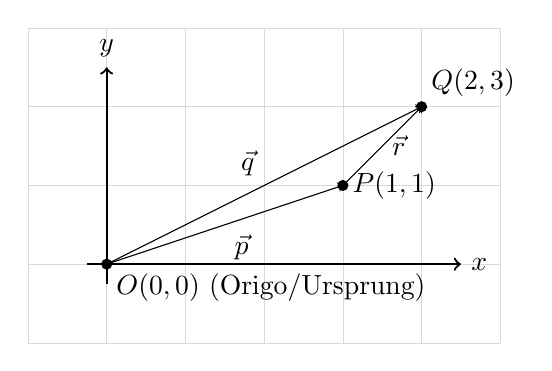
\begin{tikzpicture}
		% Draw grid
		\draw[help lines, color=gray!30] (-1,-1) grid (5,3);
		
		% Draw axes
		\draw[thick,->] (-0.25,0) -- (4.5,0) node[right] {$x$};
		\draw[thick,->] (0,-0.25) -- (0,2.5) node[above] {$y$};
		
		% Define points
		\coordinate (O) at (0,0);
		\coordinate (P) at (3,1);
		\coordinate (Q) at (4,2);
		
		% Draw vectors
		\draw[thin,->] (O) -- (P) node[midway,below right] {$\vec{p}$};
		\draw[thin,->] (O) -- (Q) node[midway,above left] {$\vec{q}$};
		\draw[thin,->] (P) -- (Q) node[midway,right] {$\vec{r}$};
		% Draw and label points
		\fill (O) circle (2pt) node[below right] {$O (0,0)$ (Origo/Ursprung)};
		\fill (P) circle (2pt) node[right] {$P (1,1)$};
		\fill (Q) circle (2pt) node[above right] {$Q (2,3)$};
		
	\end{tikzpicture}
	
	\begin{emphbox}
		\begin{tabular}{lll}
			$\overrightarrow{p}$ &= $\overrightarrow{OP}$ &= $\overrightarrow{P}$ \\
			$ \overrightarrow{q}$ &= $\overrightarrow{OQ}$ &= $\overrightarrow{Q}$ \\
			$\overrightarrow{r}$ &= $\overrightarrow{PQ}$ &= $\overrightarrow{OQ} - 		\overrightarrow{OP} = \overrightarrow{q} - \overrightarrow{p}$
		\end{tabular}
	\end{emphbox}

	Betrag/Länge eines Vektors
	\begin{emphbox}
		\begin{tabular}{l}
			$ a = \lvert\overrightarrow{a}\rvert = \sqrt{\overrightarrow{a} {\cdot} \overrightarrow{a}} = \sqrt{a_1^2 + a_2^2 + a_3^2} $
		\end{tabular}
	\end{emphbox}

	Nullvektor
	\begin{emphbox}
		\begin{tabular}{cc}
			$ \lvert\overrightarrow{0}\rvert = 0 $ & Richtung undefiniert, Länge = 0 \\
			$ 0 \cdot \overrightarrow{a} = \overrightarrow{0} $ \\
			$ \lambda \cdot \overrightarrow{0} = \overrightarrow{0} $
		\end{tabular}
	\end{emphbox}
	
	Rechenregeln
	\begin{emphbox}
		\begin{tabular}{l|l}
			Vektoraddition/-subtraktion & 	Multiplikation mit Skalar \\
			$\overrightarrow{a} \pm \overrightarrow{b} = \begin{bmatrix} a_1 \pm b_1 \\ a_2 \pm b_2 \\ a_3 \pm b_3 \end{bmatrix} $ & $
			\lambda {\cdot} \overrightarrow{a} = \begin{bmatrix} \lambda {\cdot} a_1 \\ \lambda {\cdot} a_2 \\ \lambda {\cdot} a_3 \end{bmatrix} $ \\
			& $ 1 \cdot \overrightarrow{a} = \overrightarrow{a} $ \\
			& $ -1 \cdot \overrightarrow{a} = -\overrightarrow{a} $
		\end{tabular}
		\begin{tabular}{lll}
			\text{Kommutativgesetz:} & $ \overrightarrow{a} + \overrightarrow{b} $ &
				$ = \overrightarrow{b} + \overrightarrow{a} $ \\
			\text{Assoziativgesetz:} & $ (\overrightarrow{a} + \overrightarrow{b}) + \overrightarrow{c} $ &
				$ = \overrightarrow{a} + (\overrightarrow{b} + \overrightarrow{c}) $ \\
			\text{Distributivgesetz:} & $ \lambda {\cdot} (\overrightarrow{a} + \overrightarrow{b}) $ & 
				$ = \lambda {\cdot} \overrightarrow{a} + \lambda {\cdot} \overrightarrow{b} $
		\end{tabular}
	\end{emphbox}

	Einheitsvektor
	\begin{emphbox}
		\begin{tabular}{ccc}
	 		$ \hat{a} = \frac{\overrightarrow{a}}{|\overrightarrow{a}|} $ &
	 		$|\hat{a}| = 1 $ & Richtung von $\overrightarrow{a}$, Länge = 1
		\end{tabular}
	\end{emphbox}
	- markiert mit Zirkumflex
	
	Normalenvektor

	Steht orthogonal auf einer Geraden, Kurve oder Ebene

	Normaleneinheitsvektor
	\begin{emphbox}
		\begin{tabular}{cc}
			$\overrightarrow{n_0} = \frac{\overrightarrow{n}}{|\overrightarrow{n}|}$ &
	 		$|\overrightarrow{n_0}| = 1 $
		\end{tabular}
	\end{emphbox}
	Einheitsvektor des Normalenvektors $\overrightarrow{n}$
\end{sectionbox}

\begin{sectionbox}
	Skalarprodukt (Punktprodukt, inneres Produkt)
	\begin{emphbox}
%		\begin{tabular}{{l@{\hspace{3em}}c@{\hspace{3em}}l}
		\setlength\tabcolsep{1.5pt} % default value: 6pt
		\begin{tabular}{lcl}
			\text{Geom. Form:} & $ \overrightarrow{a} {\cdot} \overrightarrow{b} $ & $ = \lvert \overrightarrow{a} \rvert {\cdot} |\overrightarrow{b}| {\cdot} \cos \alpha $ \\

			\text{Koord.form:} & $ \overrightarrow{a} {\cdot} \overrightarrow{b} $ &= $ \begin{bmatrix} a_1 \\ a_2 \\ a_3 \end{bmatrix} {\cdot} \begin{bmatrix} b_1 \\ b_2 \\ b_3 \end{bmatrix} = a_1 {\cdot} b_1 + a_2 {\cdot} b_2 + a_3 {\cdot} b_3 $
		\end{tabular}
		\begin{tabular}{lcl}

			\text{Senkr. Vekt.:} & $ \overrightarrow{a} \perp \overrightarrow{b}$ & $\Leftrightarrow \overrightarrow{a} {\cdot} \overrightarrow{b} = 0 $ \\

			\text{Kommutativgesetz:} & $ \overrightarrow{a} {\cdot} \overrightarrow{b}$ &= $\overrightarrow{b} {\cdot} \overrightarrow{a}$ \\

			\text{Assoziativgesetz:} & $(\lambda {\cdot} \overrightarrow{a}) {\cdot} \overrightarrow{b}$ &= $\lambda {\cdot} (\overrightarrow{a} {\cdot} \overrightarrow{b})$ \\

			\text{Distributivgesetz:} &	$\overrightarrow{a} {\cdot} (\overrightarrow{b} {+} \overrightarrow{c})$ &= $\overrightarrow{a} {\cdot} \overrightarrow{b} + \overrightarrow{a} {\cdot} \overrightarrow{c}$
		\end{tabular}
	\end{emphbox}

	Kreuzprodukt (Vektorprodukt, äusseres Produkt)
	\begin{emphbox}
	\setlength\tabcolsep{1.5pt} % default value: 6pt
		\begin{tabular}{lcl}
			\text{Geom. Form:} & 
			$\overrightarrow{a} {\times} \overrightarrow{b}$ &= $|\overrightarrow{a}| {\cdot} |\overrightarrow{b}| {\cdot} \sin \alpha
			{\cdot} \overrightarrow{n}$ \\

			\text{Koord.form:} & $\overrightarrow{a} {\times} \overrightarrow{b}$ &= $\begin{bmatrix} a_1 \\ a_2 \\ a_3 \end{bmatrix} {\times} \begin{bmatrix} b_1 \\ b_2 \\ b_3 \end{bmatrix} = \begin{bmatrix} a_2 {\cdot} b_3 - a_3 {\cdot} b_2 \\ a_3 {\cdot} b_1 - a_1 {\cdot} b_3 \\ a_1 {\cdot} b_2 - a_2 {\cdot} b_1 \end{bmatrix}$
			
		\end{tabular}
		\begin{tabular}{lcl}

			\text{nicht kommutativ!:} &	$\overrightarrow{a} \times \overrightarrow{b}$ & $= -(\overrightarrow{b} \times \overrightarrow{a})$ \\

			\text{Distributivgesetz:} &	$\overrightarrow{a} \times (\overrightarrow{b} + \overrightarrow{c})$ &= $\overrightarrow{a} \times \overrightarrow{b} + \overrightarrow{a} \times \overrightarrow{c}$ \\

			\text{Alt. Schreibweisen:} & $\overrightarrow{a} \times \overrightarrow{b}$ & $\equiv \overrightarrow{a} \wedge \overrightarrow{b} \equiv	[\overrightarrow{a}, \overrightarrow{b}]$
		\end{tabular}
		
	\end{emphbox}
	mit: $\overrightarrow{n}$: Einheitsvektor senkrecht zu $\overrightarrow{a}$ und $\overrightarrow{b}$
	Kreuzprodukt bildet ein Rechtssystem. Rechte-Hand-Regel: x: Daumen, y: Zeigefinger (abgespreizt), z: Mittelfinger

%	\begin{emphbox}
%	\begin{align*}
%		\text{mit: \overrightarrow{n}: Einheitsvektor senkrecht zu \overrightarrow{a} und \overrightarrow{b} }
%		\end{align*}
%	\end{emphbox}
	
\end{sectionbox}
